\documentclass[svgnames]{beamer}

\usepackage[utf8]{inputenc} % Indica cuál es la codificación de este archivo
\usepackage[spanish]{babel} % Indica el idioma en que está escrito el documento
\usepackage{fancybox}
\usepackage{graphicx}
\usepackage{amssymb} % Fuentes y símbolos adicionales (por AMS)
\usepackage{amsmath} % Mejoras a entornos matemáticos y extras (por AMS)
\usepackage{mathtools} % Correcciones a amsmath y funcionalidades extras

\usepackage{listings} % Permite ingresar código fuente de software

\lstset{ % Defino el formato de bloques de código fuente
  inputencoding=utf8, % Indico la codificación de los archivos de entrada
  %extendedchars=true, % Extiendo los caracteres
  % Escapeo caracteres especiales
  literate={¡}{{!`}}1 {¿}{{?`}}1 {á}{{\'a}}1 {é}{{\'e}}1 {í}{{\'i}}1 {ó}{{\'o}}1 {ú}{{\'u}}1 {ñ}{{\~n}}1,
  showstringspaces=false, % Indica si muestra los espacios dentro de strings
  numbers=left, % Posición en que se muestran los números de línea
  numberstyle=\tiny\color{gray}, % Estilo de los números de línea
  breaklines=true, % Se parten las líneas que exceden del ancho del documento
  frame=single, % Formato del marco del entorno
  backgroundcolor=\color{gray!5}, % Color de fondo
  basicstyle=\ttfamily\footnotesize, % Estilo de base (familia, tamaño, color)
}

\lstdefinestyle{latex}{
  tabsize=4,
  language=[LaTeX]TeX,
  keywordstyle=\color{DarkGreen}, % Estilo de las palabras reservadas
  stringstyle=\color{DarkBlue}, % Estilo de los strings
  commentstyle=\color{DarkGray}, % Estilo de los comentarios
}

\usepackage{hyperref}

% Beamer settings

\beamertemplatenavigationsymbolsempty

\AtBeginSection[]{
  \begin{frame}
    \vfill
    \centering
    \begin{beamercolorbox}[sep=8pt,center,shadow=true,rounded=true]{title}
      \usebeamerfont{title}\insertsectionhead\par%
    \end{beamercolorbox}
    \vfill
  \end{frame}
}

% Document Properties

\title{Herramientas libres para crear documentos de alta calidad}
\subtitle{Algo de {\LaTeX} y Markdown}
\author{Ezequiel ``Pampa'' Pérez Dittler}
\date{Semana LUGFI, Agosto de 2016}

\begin{document}

\frame{\titlepage}

\section{LUGFI}

\begin{frame}
  \frametitle{¿Qué es LUGFI?}

  Es el grupo de usuarios y desarrolladores de software libre y abierto de la Facultad de Ingeniería de la UBA

  Acrónimo recursivo:

  LUGFI Usa GNU/Linux en la Facultad de Ingeniería
\end{frame}

\section{Un poco de \LaTeX}

\begin{frame}
  \frametitle{¿Qué es \LaTeX?}
  \begin{itemize}
    \item Es un sistema de composición de textos
    \item Orientado a la creación de documentos con alta calidad tipográfica
    \item Muy popular en el entorno académico, especialmente entre matemáticos, físicos, químicos e informáticos
    \item Es un conjunto de macros de \TeX
    \item Es un lenguaje de maquetación (similar a HTML)
  \end{itemize}
\end{frame}

\begin{frame}
  \frametitle{¿Por qué usar \LaTeX?}
  \begin{itemize}
    \item Formato de archivo estables (en Word existen .doc y .docx)
    \item Fórmulas matemáticas de alta calidad
    \item Extensible con multitud de paquetes
    \item Permite centrarse en el contenido, no en la presentación
    \begin{itemize}
      \item La presentación se puede cambiar con multitud de plantillas
    \end{itemize}
  \end{itemize}
\end{frame}

\begin{frame}
  \frametitle{¿Cómo usar \LaTeX?}
  \framesubtitle{En forma local}
  Distribución \LaTeX
  \begin{itemize}
    \item Linux: TeX Live
    \item Windows: MiKTeX
    \item MacOS: MacTex
  \end{itemize}

  Editor de texto
  \begin{itemize}
    \item Editor de texto plano favorito (por ejemplo, Bloc de notas)
    \item TeXStudio
    \item Texmaker
    \item LyX
  \end{itemize}
\end{frame}

\begin{frame}
  \frametitle{¿Cómo usar \LaTeX?}
  \framesubtitle{En línea}
  No requiere instalar nada, sólo se necesita un navegador de internet.
  \begin{itemize}
    \item Overleaf: www.overleaf.com
    \item ShareLaTeX: www.sharelatex.com
  \end{itemize}
\end{frame}

\begin{frame}
  \frametitle{¡Hola Mundo!}
  \begin{columns} 
    \column{0.5\textwidth}\centering
      Código\\[.2cm]
      \lstinputlisting[style=latex]{hola-mundo/hola-mundo.tex}
    \column{0.5\textwidth}\centering
      Resultado\\[.2cm]
      \shadowbox{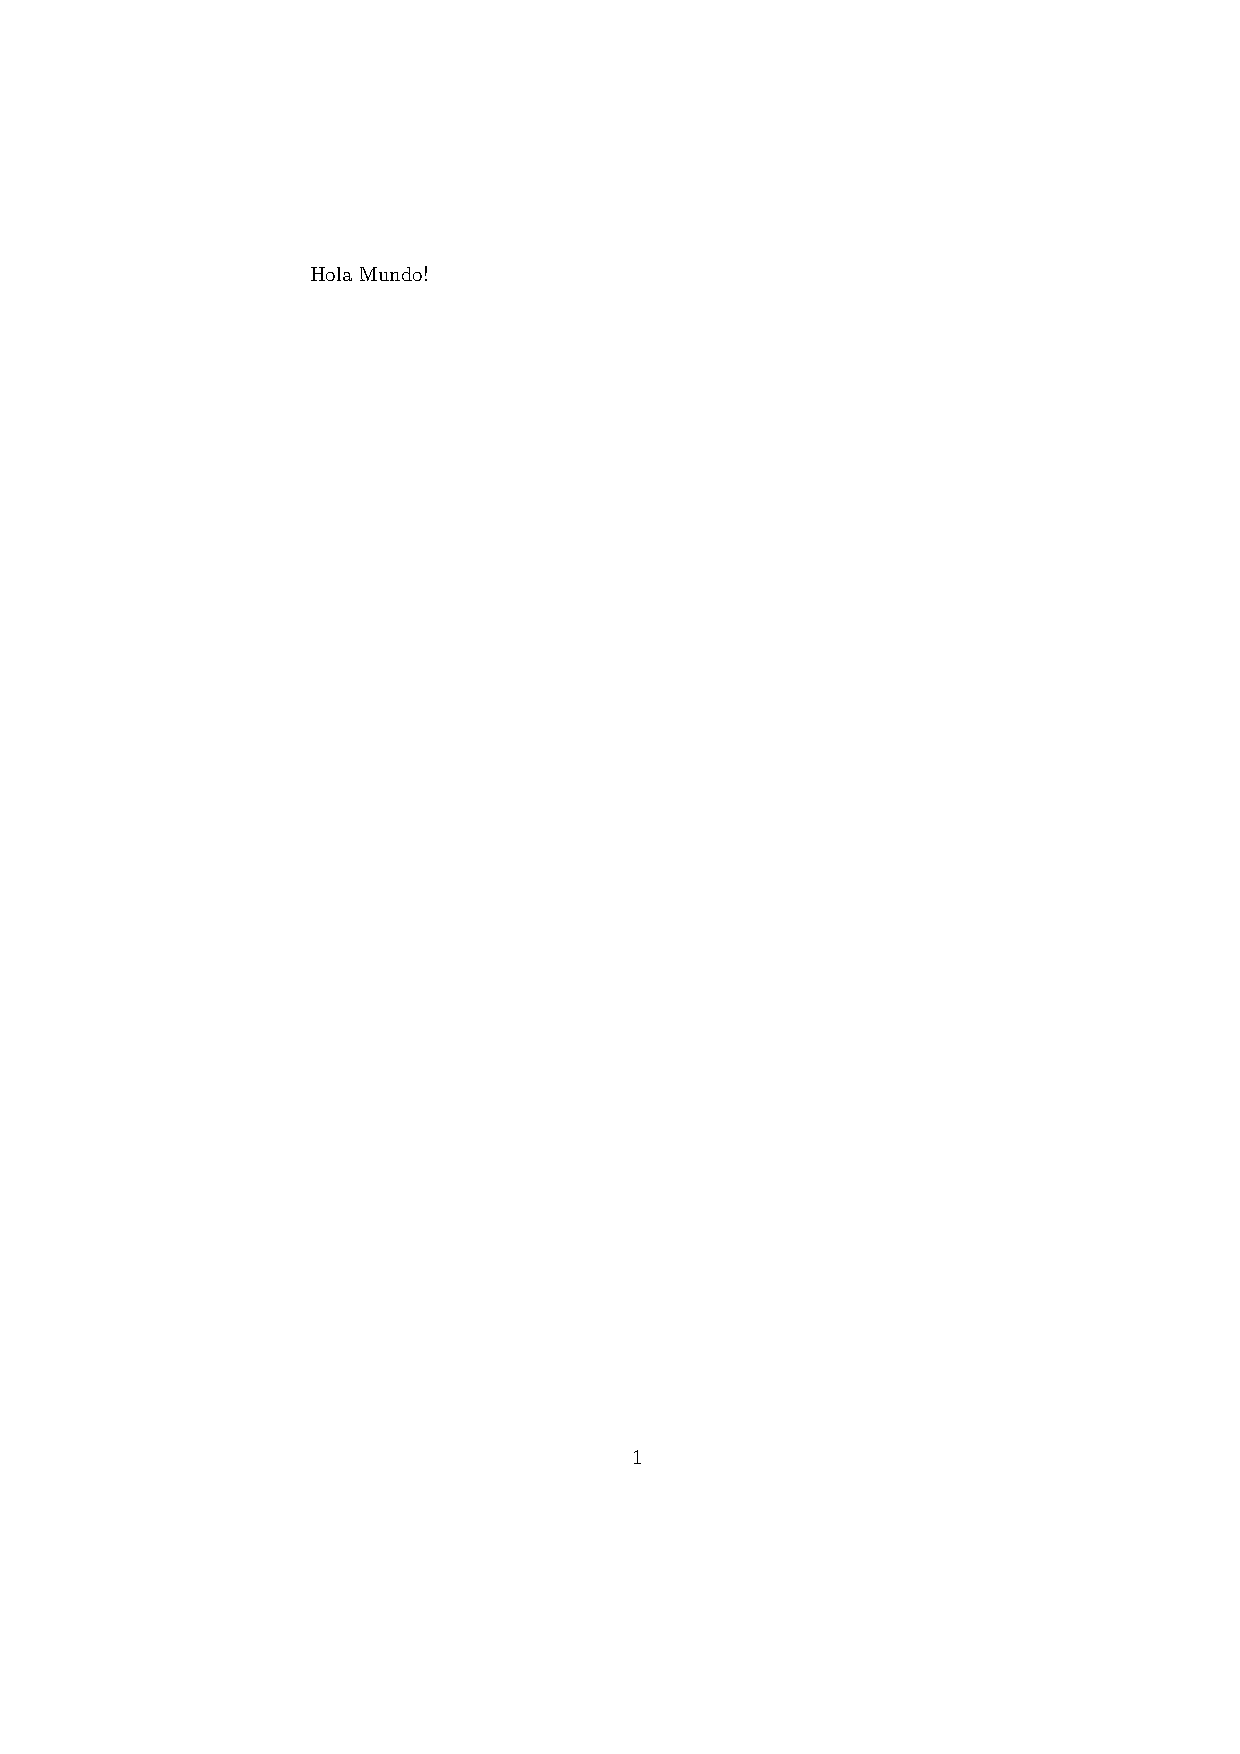
\includegraphics[height=0.8\textheight]{hola-mundo/hola-mundo.pdf}}
  \end{columns}
\end{frame}

\begin{frame}
  \frametitle{Estructura del documento}
  \begin{columns} 
    \column{0.5\textwidth}\centering
      \lstinputlisting[style=latex]{estructura/estructura.tex}
    \column{0.5\textwidth}\centering
      \begin{itemize}
        \item Preámbulo
        \begin{itemize}
          \item Inclusión y configuración de paquetes
          \item Configuración del documento
          \item Propiedades del documento
        \end{itemize}
        \item Contenido del documento
        \item Fin del documento
        \begin{itemize}
          \item Todo lo que se inserte aquí no tendrá efecto alguno tanto en la configuración como en el contenido
        \end{itemize}
      \end{itemize}
  \end{columns}
\end{frame}

\begin{frame}
  \frametitle{La codificación del caracteres del siglo XXI es: UTF-8}
  \begin{columns} 
    \column{0.5\textwidth}\centering
      \lstinputlisting[style=latex]{hola-mundo-utf/hola-mundo.tex}
    \column{0.5\textwidth}\centering
      Resultado\\[.2cm]
      \shadowbox{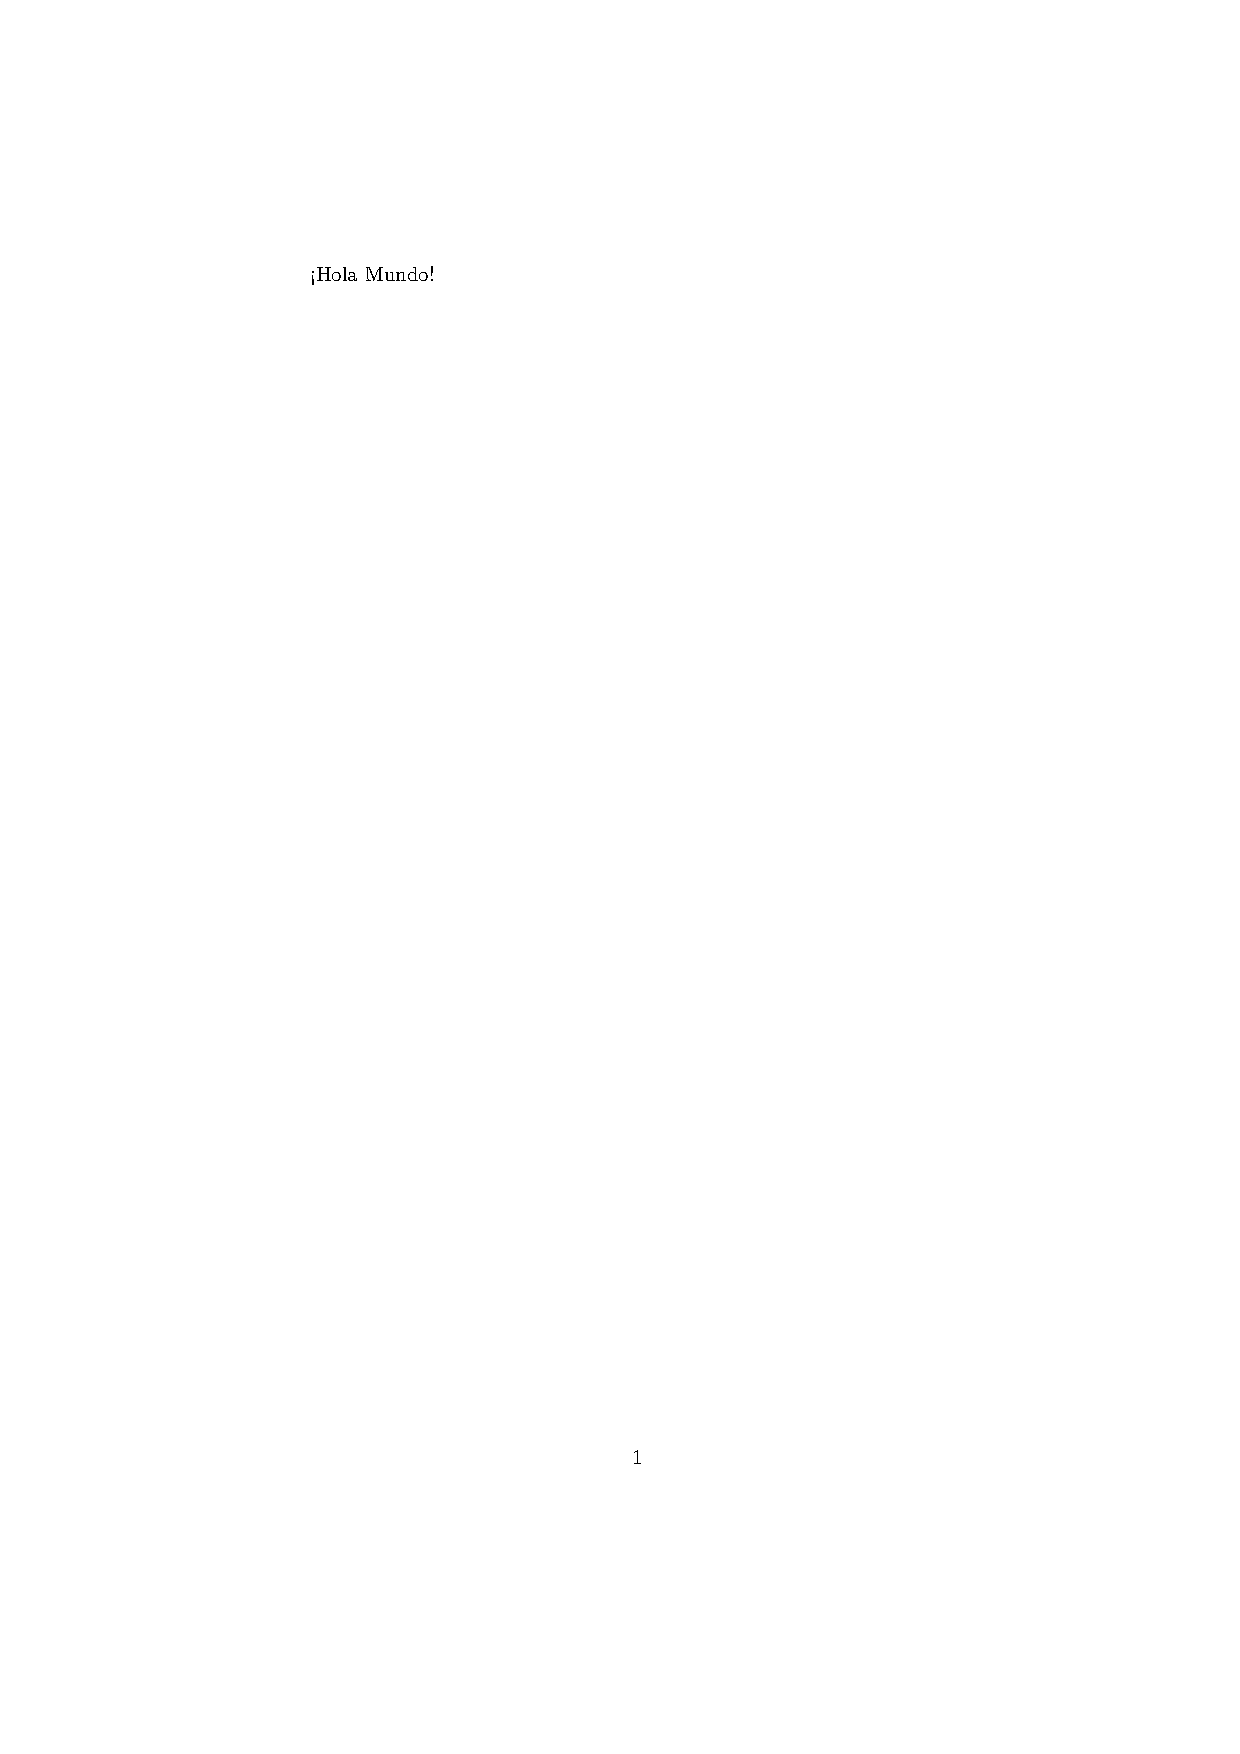
\includegraphics[height=0.7\textheight]{hola-mundo-utf/hola-mundo.pdf}}
  \end{columns}
\end{frame}

\begin{frame}
  \frametitle{¿La fuente debe ser de 12pt? ¿Hoja A4?}
  \centering
  \lstinputlisting[style=latex]{tamanios/hola-mundo.tex}
\end{frame}

\begin{frame}
  \frametitle{Ordenando en secciones}
  \begin{columns} 
    \column{0.6\textwidth}\centering
      \lstinputlisting[style=latex]{secciones/secciones.tex}
    \column{0.4\textwidth}\centering
      Resultado\\[.2cm]
      \shadowbox{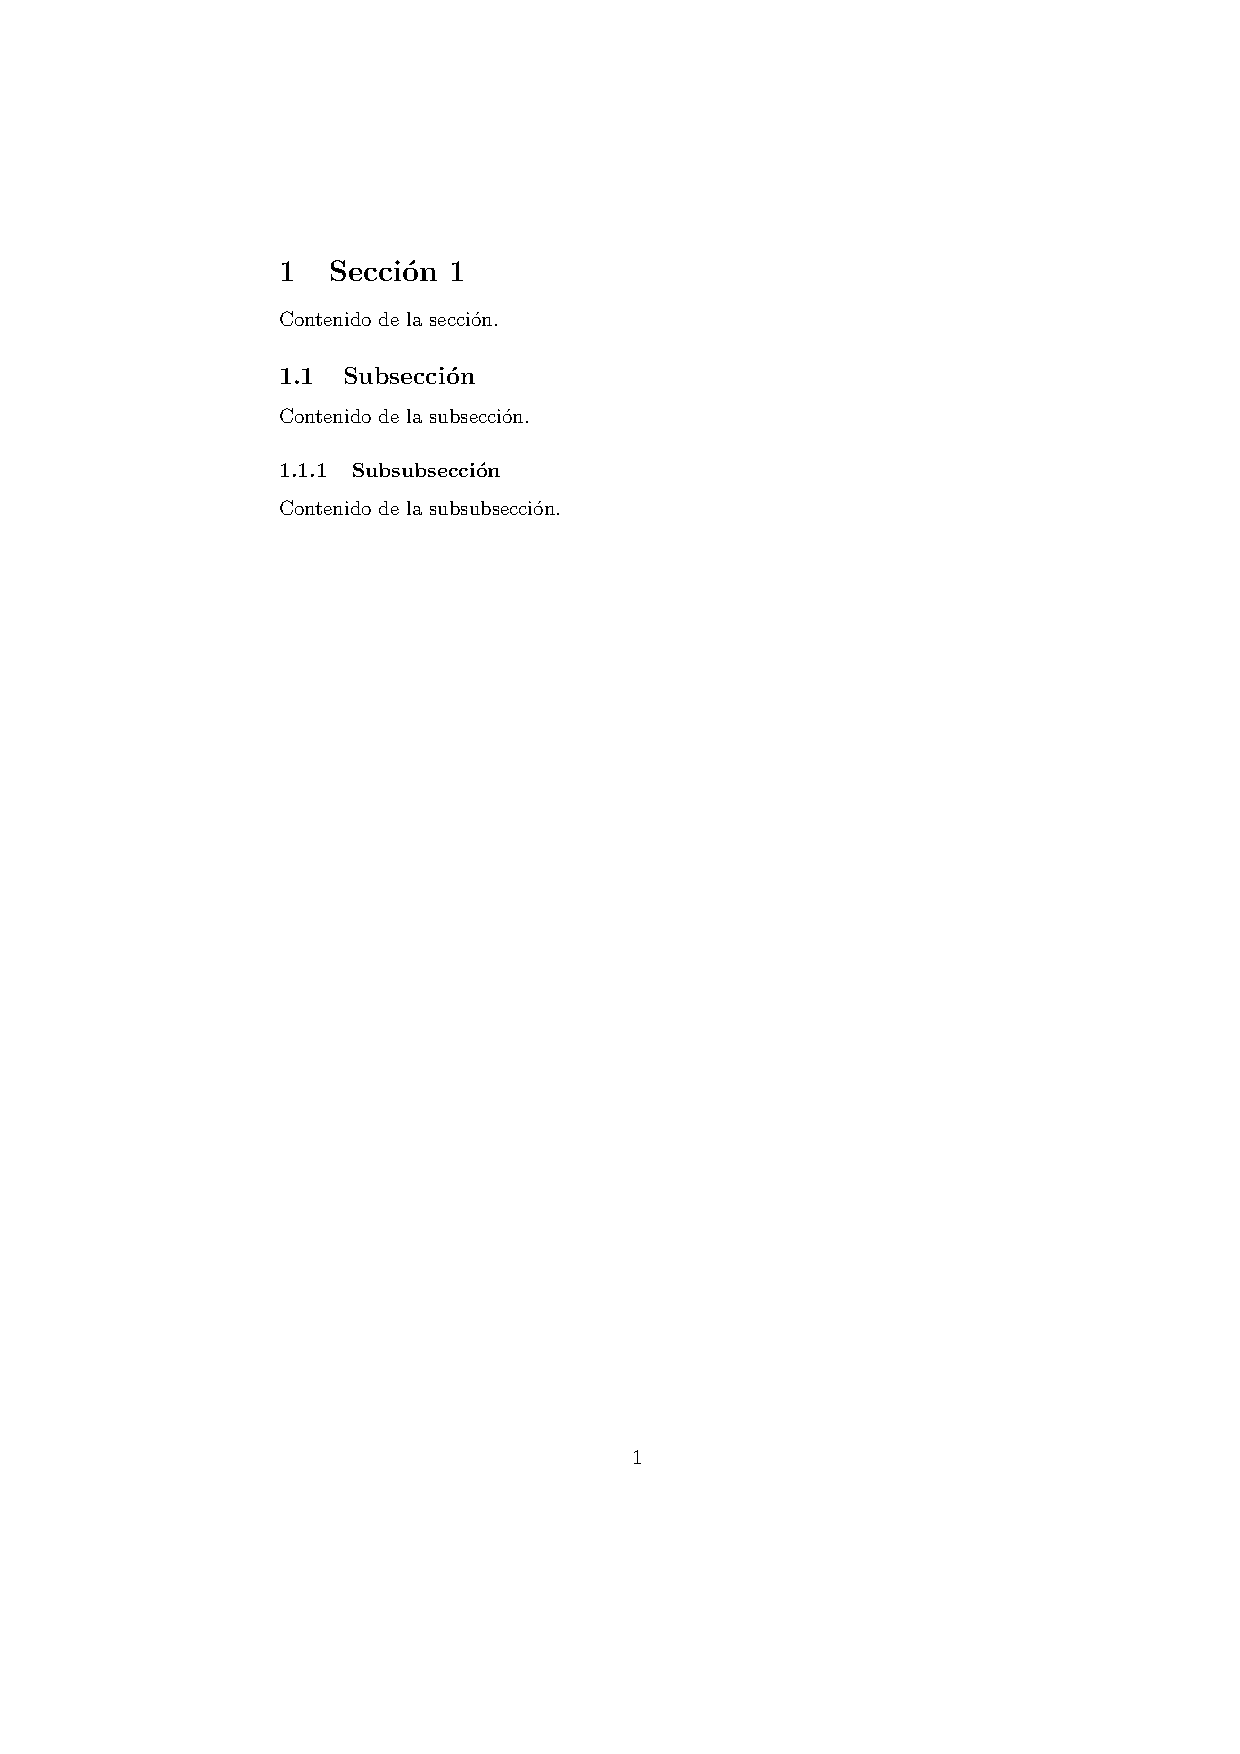
\includegraphics[height=0.7\textheight]{secciones/secciones.pdf}}
  \end{columns}
\end{frame}

\end{document}
